% !TEX program = lualatex
\documentclass[aspectratio=43,professionalfonts,handout]{beamer}
\usepackage{beamer_template}

\newcommand{\LectureNum}{1}
\newcommand{\LectureTitle}{累乗根・指数の拡張（１）}
\newcommand{\TextPages}{p.\,102-104}
\newcommand{\NextTopic}{累乗根・指数の拡張（２）}
\newcommand{\NextPages}{p.\,104-106}
\newcommand{\CourseName}{基礎数学B}
\renewcommand{\TermName}{後期}

\begin{document}

% -----------------------------------------------
% スライド1: 表紙＋目標＋用語・定義
% -----------------------------------------------
\begin{frame}{\CourseName\quad 第\LectureNum 回「\LectureTitle 」}
  {\small \TermName\quad \TeacherName\quad ／\quad 教科書 \TextPages\quad
  \textbf{目標}：累乗根の定義と性質を理解し計算できる}

  \begin{block}{用語・定義}
  \begin{description}[labelwidth=5.5em]
    \item[\kw{n乗根}] ~
    \item[\kw{n乗根の定義（aのn乗根）}] ~
    \item[\kw{√ⁿa の表記}] ~
    \item[\kw{奇数乗根と偶数乗根の違い}] ~
  \end{description}
  \end{block}
\end{frame}

% -----------------------------------------------
% スライド2: 公式・性質
% -----------------------------------------------
\begin{frame}{公式・性質}
  \begin{block}{}
  \begin{itemize}
    \item (√ⁿa)ⁿ=a
    \item √ⁿ(aⁿ)=a（nが奇数）
    \item √ⁿ(aⁿ)=|a|（nが偶数）
    \item √ⁿa・√ⁿb=√ⁿ(ab)
    \item √ⁿa÷√ⁿb=√ⁿ(a/b)
  \end{itemize}
  \end{block}
\end{frame}

% -----------------------------------------------
% スライド3: 図・グラフ（TikZコードを手動追加）
% -----------------------------------------------
\begin{frame}{図・グラフ}
  \centering
  % TODO: 数直線上でのn乗根の位置（n=2,3,4の比較）
  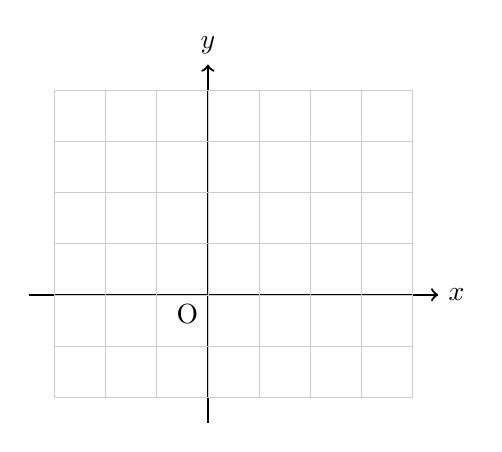
\begin{tikzpicture}[scale=0.65]
    \draw[->,thick] (-3.5,0) -- (4.5,0) node[right]{$x$};
    \draw[->,thick] (0,-2.5) -- (0,4.5) node[above]{$y$};
    \node[below left] at (0,0) {O};
    \draw[gray!40, very thin] (-3,-2) grid (4,4);
    % ここにグラフを描画
  \end{tikzpicture}
\end{frame}

% -----------------------------------------------
% スライド4: 例1→問1
% -----------------------------------------------
\begin{frame}{例1→問1}
  \begin{exampleblock}{例1) p.102（n乗根の値を求める）}
    （板書で解説）
  \end{exampleblock}

  \vfill

  \begin{block}{問1) p.102\quad 自分で解いてみよう}
    （ノートに解くこと）
  \end{block}
\end{frame}

% -----------------------------------------------
% スライド5: 例2→問2
% -----------------------------------------------
\begin{frame}{例2→問2}
  \begin{exampleblock}{例2) p.103（√ⁿa の計算）}
    （板書で解説）
  \end{exampleblock}

  \vfill

  \begin{block}{問2) p.103\quad 自分で解いてみよう}
    （ノートに解くこと）
  \end{block}
\end{frame}

% -----------------------------------------------
% まとめ
% -----------------------------------------------
\begin{frame}{まとめ}
  \begin{itemize}
    \item % TODO: まとめを記入
  \end{itemize}

  \vfill
  {\small 基本問題：201, 202, 203, 204}
\end{frame}

\end{document}
